%	-------------------------------------------------------------------------------
%
%
%
%
%
%
%
%
%	-------------------------------------------------------------------------------

%	\documentclass[10pt,xcolor=pdftex,dvipsnames,table]{beamer}
%	16:10
%	\documentclass[ aspectratio=1610, 10pt,blue,xcolor=pdftex,dvipsnames,table,handout]{beamer}
%	\documentclass[ aspectratio=1610, 10pt,blue,xcolor=pdftex,dvipsnames,table,handout,notes]{beamer}
%	16:9 
%	\documentclass[ aspectratio=169,  10pt,blue,xcolor=pdftex,dvipsnames,table,handout]{beamer}
	\documentclass[ aspectratio=169,  10pt,blue,xcolor=pdftex,dvipsnames,table,handout,notes]{beamer}
%	14:9 
%	\documentclass[ aspectratio=149,  10pt,blue,xcolor=pdftex,dvipsnames,table,handout]{beamer}
%	5:4
%	\documentclass[ aspectratio=54,   10pt,blue,xcolor=pdftex,dvipsnames,table,handout]{beamer}
%	4:3 default
%	\documentclass[ aspectratio=43, 10pt,blue,xcolor=pdftex,dvipsnames,table,handout]{beamer}
%	3:2 
% 	\documentclass[ aspectratio=32, 10pt,blue,xcolor=pdftex,dvipsnames,table,handout]{beamer}







		% Font Size
		%	default font size : 11 pt
		%	8,9,10,11,12,14,17,20
		%
		% 	put frame titles 
		% 		1) 	slideatop
		%		2) 	slide centered
		%
		%	navigation bar
		% 		1)	compress
		%		2)	uncompressed
		%
		%	Color
		%		1) blue
		%		2) red
		%		3) brown
		%		4) black and white	
		%
		%	Output
		%		1)  	[default]	
		%		2)	[handout]		for PDF handouts
		%		3) 	[trans]		for PDF transparency
		%		4)	[notes=hide/show/only]

		%	Text and Math Font
		% 		1)	[sans]
		% 		2)	[sefif]
		%		3) 	[mathsans]
		%		4)	[mathserif]


		%	---------------------------------------------------------	
		%	슬라이드 크기 설정 ( 128mm X 96mm )
		%	---------------------------------------------------------	
			\setbeamersize{text margin left=10mm}
			\setbeamersize{text margin right=10mm}

%			% Format presentation size to A4
%			\usepackage[size=a4]{beamerposter}		% A4용지 크기 사용

%			% Format presentation size to A4
%			\setlength{\paperwidth}{297mm}
%			\setlength{\paperheight}{210mm}
%			\setlength{\textwidth}{287mm}
%			\setlength{\textheight}{200mm}   



	%	========================================================== 	Package
			\usepackage{kotex}						% 한글 사용
			\usepackage{amssymb,amsfonts,amsmath}	% 수학 수식 사용
			\usepackage{color}					%
			\usepackage{colortbl}					%

			\usepackage{tikz}				% TikZ picture
			\usetikzlibrary{shapes,arrows,positioning}







		
		%	---------------------------------------------------------	
		%		유인물 출력 : 출력할대 조정해서 출력 할것
		%	---------------------------------------------------------	

			\usepackage{pgfpages}
%			\pgfpagesuselayout{2 on 1}[letterpaper]
%			\pgfpagesuselayout{4 on 1}[letterpaper]
%			\pgfpagesuselayout{8 on 1}[letterpaper]

%			\pgfpagesuselayout{resize to}[a4paper,landscape,border shrink=5mm]
%			\pgfpagesuselayout{resize to}[a4paper,border shrink=5mm]
%			\pgfpagesuselayout{2 on 1}[a4paper,border shrink=5mm]
%			----------------------------------------------------- 출력 시 설정	1
%			\pgfpagesuselayout{2 on 1}[a4paper]
%			\usecolortheme{seagull}	% 휜색
%			----------------------------------------------------- 출력 시 설정	2
			\pgfpagesuselayout{2 on 1}[a4paper,border shrink=5mm]
			\usecolortheme{dove}
%			----------------------------------------------------- 
%			\pgfpagesuselayout{4 on 1}[a4paper,border shrink=5mm]
%			\pgfpagesuselayout{8 on 1}[a4paper,border shrink=5mm]

			\usepackage{handoutWithNotes}
%			\pgfpagesuselayout{1 on 1 with notes}[a4paper,border shrink=5mm]
%			\pgfpagesuselayout{2 on 1 with notes}[a4paper,border shrink=5mm]
%			\pgfpagesuselayout{3 on 1 with notes}[a4paper,border shrink=5mm]
%			\pgfpagesuselayout{4 on 1 with notes}[a4paper,border shrink=5mm]

%			\pgfpagesuselayout{2 on 1}[letterpaper]
%			\pgfpagesuselayout{2 on 1}[letterpaper]
%			\pgfpagesuselayout{2 on 1}[letterpaper]

	%		========================================================= 	Theme

		%	---------------------------------------------------------	
		%	전체 테마
		%	---------------------------------------------------------	
		%	테마 명명의 관례 : 도시 이름
%			\usetheme{default}			%
%			\usetheme{Madrid}    		%
%			\usetheme{CambridgeUS}    	% -red, no navigation bar
			\usetheme{Antibes}			% -blueish, tree-like navigation bar

		%	----------------- table of contents in sidebar
%			\usetheme{Berkeley}		% -blueish, table of contents in sidebar
									% 개인적으로 마음에 듬
%			\usetheme{Marburg}			% - sidebar on the right
%			\usetheme{Hannover}		% 왼쪽에 마크
%			\usetheme{Berlin}			% - navigation bar in the headline
%			\usetheme{Szeged}			% - navigation bar in the headline, horizontal lines
%			\usetheme{Malmoe}			% - section/subsection in the headline

%			\usetheme{Singapore}
%			\usetheme{Amsterdam}

		%	---------------------------------------------------------	
		%	색 테마
		%	---------------------------------------------------------	
%			\usecolortheme{albatross}	% 바탕 파란
%			\usecolortheme{crane}		% 전체적으로 노란색 계열
%			\usecolortheme{beetle}		% 바탕 회색
%			\usecolortheme{dove}		% 전체적으로 흰색 ( 출력용으로 적합 : 잉크 절약)
%			\usecolortheme{fly}		% 전체적으로 회색
			\usecolortheme{seagull}	% 휜색
%			\usecolortheme{wolverine}	& 제목이 노란색
%			\usecolortheme{beaver}

		%	---------------------------------------------------------	
		%	Inner Color Theme 			내부 색 테마 ( 블록의 색 )
		%	---------------------------------------------------------	

%			\usecolortheme{rose}		% 흰색
%			\usecolortheme{lily}		% 색 안 칠한다
%			\usecolortheme{orchid} 	% 진하게

		%	---------------------------------------------------------	
		%	Outter Color Theme 		외부 색 테마 ( 머리말, 고리말, 사이드바 )
		%	---------------------------------------------------------	

%			\usecolortheme{whale}		% 진하다
%			\usecolortheme{dolphin}	% 중간
%			\usecolortheme{seahorse}	% 연하다

		%	---------------------------------------------------------	
		%	Font Theme 				폰트 테마
		%	---------------------------------------------------------	
%			\usfonttheme{default}		
			\usefonttheme{serif}			
%			\usefonttheme{structurebold}			
%			\usefonttheme{structureitalicserif}			
%			\usefonttheme{structuresmallcapsserif}			



		%	---------------------------------------------------------	
		%	Inner Theme 				
		%	---------------------------------------------------------	

%			\useinnertheme{default}
			\useinnertheme{circles}		% 원문자			
%			\useinnertheme{rectangles}		% 사각문자			
%			\useinnertheme{rounded}			% 깨어짐
%			\useinnertheme{inmargin}			




		%	---------------------------------------------------------	
		%	이동 단추 삭제
		%	---------------------------------------------------------	
%			\setbeamertemplate{navigation symbols}{}

		%	---------------------------------------------------------	
		%	문서 정보 표시 꼬리말 적용
		%	---------------------------------------------------------	
%			\useoutertheme{infolines}


			
	%	---------------------------------------------------------- 	배경이미지 지정
%			\pgfdeclareimage[width=\paperwidth,height=\paperheight]{bgimage}{./fig/Chrysanthemum.jpg}
%			\setbeamertemplate{background canvas}{\pgfuseimage{bgimage}}

		%	---------------------------------------------------------	
		% 	본문 글꼴색 지정
		%	---------------------------------------------------------	
%			\setbeamercolor{normal text}{fg=purple}
%			\setbeamercolor{normal text}{fg=red!80}	% 숫자는 투명도 표시


		%	---------------------------------------------------------	
		%	itemize 모양 설정
		%	---------------------------------------------------------	
%			\setbeamertemplate{items}[ball]
%			\setbeamertemplate{items}[circle]
%			\setbeamertemplate{items}[rectangle]


		%	---------------------------------------------------------	
		%	상자 모양새 설정
		%	---------------------------------------------------------	
%			\setbeamertemplate{blocks}[rounded,shadow=true]
%			\begin{block}
%			\begin{theorem}
%			\begin{lemma}
%			\begin{proof}
%			\begin{corollary}
%			\begin{example}
%			\begin{exampleblock}
%			\begin{alertblock}




		\setbeamercovered{dynamic}


		%	---------------------------------------------------------	
		%		Background 
		%	---------------------------------------------------------	

%			\beamersetaveragebackground{yellow!20}
%			\beamertemplatesolidbackgroundcolor{yellow!20}
%			\beamertemplategridbackground [5mm]




		% --------------------------------- 	문서 기본 사항 설정
		\setcounter{secnumdepth}{1} 		% 문단 번호 깊이
		\setcounter{tocdepth}{1} 			% 문단 번호 깊이




% ------------------------------------------------------------------------------
% Begin document (Content goes below)
% ------------------------------------------------------------------------------
	\begin{document}
	

			\title{TikZ picture Shape Librery}
			\author{김대희}
			\date{2015년 7월}



	%	==========================================================
	%		타이틀 페이지 출력
	%	----------------------------------------------------------
		\begin{frame}[plain]
		\titlepage
		\note[item]{}
		\end{frame}








	%	==========================================================
	%		Predefined Shapes
	%	----------------------------------------------------------

	%	----------------------------------------------------------
	%		circle
	%	----------------------------------------------------------

	%	----------------------------------------------------------
	%		rectangle
	%	----------------------------------------------------------

	%	----------------------------------------------------------
	%		diamond
	%	----------------------------------------------------------


	%	----------------------------------------------------------
	%		ellipse
	%	----------------------------------------------------------


	%	----------------------------------------------------------
	%		trapezium
	%	----------------------------------------------------------


	%	----------------------------------------------------------
	%		semicircle
	%	----------------------------------------------------------



	%	----------------------------------------------------------
	%		regular polygon
	%	----------------------------------------------------------


	%	----------------------------------------------------------
	%		star
	%	----------------------------------------------------------


	%	----------------------------------------------------------
	%		kite
	%	----------------------------------------------------------


	%	----------------------------------------------------------
	%		dart
	%	----------------------------------------------------------



	%	----------------------------------------------------------
	%		circular sector
	%	----------------------------------------------------------



	%	----------------------------------------------------------
	%		cylinder
	%	----------------------------------------------------------





	%	==========================================================
	%		Symbol Shapes
	%	----------------------------------------------------------


	%	----------------------------------------------------------
	%		forbidden sign
	%	----------------------------------------------------------


	%	----------------------------------------------------------
	%		magnifying glass
	%	----------------------------------------------------------


	%	----------------------------------------------------------
	%		cloud
	%	----------------------------------------------------------


	%	----------------------------------------------------------
	%		starburst
	%	----------------------------------------------------------


	%	----------------------------------------------------------
	%		signal
	%	----------------------------------------------------------



	%	----------------------------------------------------------
	%		tape
	%	----------------------------------------------------------



	%	==========================================================
	%		Arrow Shapes
	%	----------------------------------------------------------


	%	----------------------------------------------------------
	%		single arrow
	%	----------------------------------------------------------


	%	----------------------------------------------------------
	%		double arrow
	%	----------------------------------------------------------



	%	----------------------------------------------------------
	%		arrow box
	%	----------------------------------------------------------



	%	==========================================================
	%		Shapes with Multiple Text Parts
	%	----------------------------------------------------------


	%	----------------------------------------------------------
	%		circle split
	%	----------------------------------------------------------



	%	----------------------------------------------------------
	%		circle solidus
	%	----------------------------------------------------------


	%	----------------------------------------------------------
	%		ellipse split
	%	----------------------------------------------------------


	%	----------------------------------------------------------
	%		rectangle split
	%	----------------------------------------------------------



	%	==========================================================
	%		Callout Shapes
	%	----------------------------------------------------------


	%	----------------------------------------------------------
	%		rectangle callout
	%	----------------------------------------------------------



	%	----------------------------------------------------------
	%		ellipse callout
	%	----------------------------------------------------------


	%	----------------------------------------------------------
	%		cloud callout
	%	----------------------------------------------------------




	%	==========================================================
	%		Miscellaneous Shapes
	%	----------------------------------------------------------


	%	----------------------------------------------------------
	%		cross out
	%	----------------------------------------------------------


	%	----------------------------------------------------------
	%		strike out
	%	----------------------------------------------------------


	%	----------------------------------------------------------
	%		rounded rectangle
	%	----------------------------------------------------------


	%	----------------------------------------------------------
	%		chamfered rectangle
	%	----------------------------------------------------------





		\begin{frame}[t]
		\frametitle{기본 그리기 명령 : draw}

			\begin{block}{Draw}
			\begin{itemize}
			\item[] 	\textbackslash draw ( \_ , \_ ) $--$ ( \_ , \_ ) ;
			\item[] 	\textbackslash draw [ verythin, red ] ( \_ , \_ ) \_\_ ( \_ , \_ ) ;
			\end{itemize}
			\end{block}

		\note[item]{ }

			\begin{block}{선 굵기}
			\begin{enumerate}
			\item 	very thin
			\item 	very thick
			\item 	ultra thin
			\item 	ultra thick
			\item 	thin
			\item 	thick
			\item 	semithick
			\end{enumerate}
			\end{block}


		\end{frame}


	%	==========================================================
	%		기본 그리기 명령 : path
	%	----------------------------------------------------------
		\begin{frame}[t]
		\frametitle{기본 그리기 명령 : path}

			\begin{block}{Path}
			\begin{itemize}
			\item[] 	\textbackslash path ( a , b )
			\item[] 	\textbackslash path ( $\alpha$ : rim )
					\begin{description}[1234567890]
					\item[$\alpha$] : angle
					\item[rim] : radius
					\end{description}

			\end{itemize}
			\end{block}

		\note[item]{ }

		\end{frame}


	%	==========================================================
	%		기본 그리기 명령 : path[line]
	%	----------------------------------------------------------
		\begin{frame}[t]
		\frametitle{기본 그리기 명령 : path [ line ]}

			\begin{block}{Path [ line ]}
			\end{block}


			\begin{example}
			\begin{itemize}
				\item[] \textbackslash tikzstyle\{line\} = [ draw , -latex]
				\item[] \textbackslash begin\{tikzpicture\}
				\item[] \textbackslash path [line] (0,0)--(1,0);
				\item[] \textbackslash end\{tikzpicture\}
			\end{itemize}
			\end{example}

			\begin{example}
				\tikzstyle{line} = [ draw , -latex]
				\begin{tikzpicture}
			 	\path [line] (0,0)--(1,0);
				\end{tikzpicture}
			\end{example}



		\note[item]{ }

		\end{frame}

	%	==========================================================
	%		기본 그리기 명령 : 예제
	%	----------------------------------------------------------
		\begin{frame}[t]
		\frametitle{기본 그리기 명령}

			\begin{example}
			\begin{itemize}
			\item[] 	\textbackslash begin \{ tikzpicture\}
			\item[] 	\% Define the points of a regular pentagon
			\item[] 	\textbackslash path (0,0) coordinate (origin) ;
			\item[] 	\textbackslash path (0 : 1cm) coordinate (P0 ) ;
			\item[] 	\textbackslash path (1*72 : 1cm) coordinate (P1 ) ;
			\item[] 	\textbackslash path (2*72 : 1cm) coordinate (P2 ) ;
			\item[] 	\textbackslash path (3*72 : 1cm) coordinate (P3 ) ;
			\item[] 	\textbackslash path (4*72 : 1cm) coordinate (P4 ) ;
			\item[] 	\% Define the points of a regular pentagon
			\item[] 	\textbackslash draw (p0) $--$ (p1) $--$ (p2) $--$ (p3) $--$ (p4) $--$ cycle;
			\item[] 	\% Add spokes
			\item[] 	\textbackslash draw (origin) $--$ (p0) (origin) $--$ (p1) 
								(origin) $--$ (p2) (origin) $--$ (p3) (origin) $--$ (p4);
			\item[] 	\textbackslash end \{tikzpicture \}
			\end{itemize}
			\end{example}

		\note[item]{ }

		\end{frame}

		\begin{frame}[t]
		\frametitle{기본 그리기 명령}

			\begin{example}
				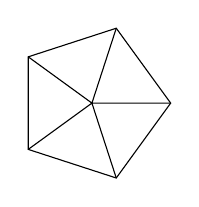
\begin{tikzpicture}
			 	\path (0,0) coordinate (origin) ;
				\path (0 : 1cm) 	coordinate (p0) ;
				\path (1*72 : 1cm) coordinate (p1) ;
				\path (2*72 : 1cm) coordinate (p2) ;
				\path (3*72 : 1cm) coordinate (p3) ;
				\path (4*72 : 1cm) coordinate (p4) ;
				\draw (p0)--(p1)--(p2)--(p3)--(p4)--cycle;
				\draw (origin)--(p0) (origin)--(p1) (origin)--(p2) (origin)--(p3) (origin)--(p4);
				\end{tikzpicture}
			\end{example}

		\note[item]{ }

		\end{frame}





	%	==========================================================
	%		기본 그리기 명령 : node
	%	----------------------------------------------------------
		\begin{frame}[t]
		\frametitle{기본 그리기 명령 : node}

			\begin{block}{node}
			\end{block}


		\note[item]{}
		\end{frame}




	%	==========================================================
	%		기본 그리기 명령 : node[block]
	%	----------------------------------------------------------
		\begin{frame}[t]
		\frametitle{기본 그리기 명령 : node[block]}

			\begin{block}{node}
			\begin{itemize}
			\item[] 	\textbackslash tikzstyle \{block\} = [ rectangle, draw, text width=6em, text height=1em]
			\item[] 	\textbackslash tikzstyle\{line\} = [ draw , -latex]
			\item[] 	\textbackslash begin\{tikzpicture\}[node distance = 8em and 2em, auto]

			\item[] 	\textbackslash node [block] (b0) 				{ 0000 }
			\item[] 	\textbackslash node [block, left of=b0 ] (b1) 	{ 1111 }
			\item[] 	\textbackslash node [block, right of=b0 ] (b2) 	{ 1111 }
			\item[] 	\textbackslash node [block, below of=b0 ] (b3) 	{ 1111 }
			\item[] 	\textbackslash node [block, below of=b3 ] (b4) 	{ 1111 }
			\item[] 	\textbackslash path [line] (b0) $--$ (b1)
			\item[] 	\textbackslash path [line] (b0) $--$ (b2)
			\item[] 	\textbackslash path [line] (b0) $--$ (b3)
			\item[] 	\textbackslash path [line] (b3) $--$ (b4)
			\item[] 	\textbackslash end\{tikzpicture\}

			\end{itemize}
			\end{block}

		\note[item]{ block스타일 정의에서 넓이}
		\note[item]{ block스타일 정의에서 높이}
		\note[item]{ line의 -retex의 의미}
		\note[item]{ block의 배치
					\begin{itemize}
					\item left
					\item right
					\item below
					\item above
					\end{itemize}

					}
		\note[item]{ distance의 8 과 2의 의미}
		\end{frame}


	%	----------------------------------------------------------
		\begin{frame}[t]
		\frametitle{기본 그리기 명령}

			\begin{block}{node}

			\tikzstyle{block} = [ rectangle, draw, text width=6em, text height=1em]
			\tikzstyle{line} = [ draw , -latex]

			\begin{tikzpicture}[node distance = 8em and 2em, auto]
			\node [block] (b0) 				{ 0000 };
			\node [block, left of=b0 ] (b1) 	{ 1111 };
			\node [block, right of=b0 ] (b2) 	{ 2222 };
			\node [block, below of=b0 ] (b3) 	{ 3333 };
			\node [block, below of=b3 ] (b4) 	{ 4444 };

			\path [line] (b0)--(b1);
			\path [line] (b0)--(b2);
			\path [line] (b0)--(b3);
			\path [line] (b3)--(b4);

			\end{tikzpicture}

			\end{block}

		\note[item]{ }
		\end{frame}



	%	==========================================================
	%		기본 그리기 명령 : node[block]
	%	----------------------------------------------------------
		\begin{frame}[t]
		\frametitle{기본 그리기 명령 : node[block]}



		\note[item]{}
		\end{frame}


	%	----------------------------------------------------------
		\begin{frame}[t]
		\frametitle{node distance}

			\begin{block}{node distance}

			\begin{itemize}
			\item[] 	\textbackslash begin\{tikzpicture\}[node distance = 8em and 2em, auto]
			\end{itemize}

			\end{block}
	
		\note[item]{ }
		\end{frame}



	%	----------------------------------------------------------
		\begin{frame}[t]
		\frametitle{positing 라이버러리 사용}

			\begin{block}{node distance}

			\begin{itemize}
			\item[] 	\textbackslash node [block, below of=b0 ] (b3) \{ 3333 \};
			\item[] 	\textbackslash node [block, below=2em of b0 ] (b3) \{ 3333 \};
			\end{itemize}

			\end{block}

			\begin{block}{xshift, yshift}

			\begin{itemize}
			\item[] 	xshift = -2em
			\item[] 	yshift = -2em
			\end{itemize}

			\end{block}

	
		\note[item]{ }

		\end{frame}



	%	==========================================================
	%		Placing Nodes
	%	----------------------------------------------------------
		\begin{frame}[plain]

			\centering
			\scalebox{4}{Placing Nodes}
	
		\note[item]{ }
		\end{frame}




	%	----------------------------------------------------------
		\begin{frame}[t]
		\frametitle{Placing Nodes}

			\begin{block}{Placing Nodes Using at syntax}
			\begin{itemize}
			\item[] 	\textbackslash node at ( $-$ , $-$ )
			\end{itemize}
			\end{block}

			\begin{block}{Placing Nodes Using Relative Placement}
			\begin{itemize}
			\item[] 	\textbackslash node [below of=$--$ ] (b3) \{ 3333 \};
			\item[] 	\textbackslash node [above of=$--$ ] (b3) \{ 3333 \};
			\item[] 	\textbackslash node [left of=$--$ ] (b3) \{ 3333 \};
			\item[] 	\textbackslash node [right of=$--$ ] (b3) \{ 3333 \};
 			\end{itemize}
			\end{block}

			\begin{block}{Placing Nodes Using Anchors}
			\begin{itemize}
			\item[] 	\textbackslash node [anchor=north west] (b3) \{ 3333 \};
			\item[] 	\textbackslash node [anchor=north ] (b3) \{ 3333 \};
			\item[] 	\textbackslash node [anchor=north east] (b3) \{ 3333 \};
			\item[] 	\textbackslash node [anchor=west] (b3) \{ 3333 \};
			\item[] 	\textbackslash node [anchor=east] (b3) \{ 3333 \};
			\item[] 	\textbackslash node [base] (b3) \{ 3333 \};
 			\end{itemize}
			\end{block}

	
		\note[item]{ }
		\end{frame}




	%	----------------------------------------------------------
		\begin{frame}[plain]

			\centering
			\scalebox{4}{Tikz Style}
	
		\note[item]{ }
		\end{frame}




	%	==========================================================
	%		영역 채우기
	%	----------------------------------------------------------
		\begin{frame}[plain]

			\centering
			\scalebox{4}{영역 색깔로 채우기}
	
		\note[item]{ }
		\end{frame}













	%	==========================================================
	%		Tikz Style
	%	----------------------------------------------------------
		\begin{frame}[t]
		\frametitle{Tikz Style}

			\begin{block}{Tikz Style}
			\begin{itemize}
			\item[] 	\textbackslash tikzstyle \{block\} = [ rectangle, draw, text width=6em, text height=1em]
			\item[] 	\textbackslash tikzstyle\{line\} = [ draw , -latex]
			\end{itemize}
			\end{block}


			\begin{block}{width, height}
			\begin{itemize}
			\item[] 	text width = 6em
			\item[] 	text height = 6em
			\item[] 	minimum width = 6em
			\item[] 	minimum height = 6em
			\end{itemize}
			\end{block}

			\begin{block}{shape}
			\begin{itemize}
			\item[] 	rectangle
			\item[] 	trapezium
			\item[] 	diamond
			\end{itemize}
			\end{block}


		\note[item]{}
		\end{frame}


	%	----------------------------------------------------------
		\begin{frame}[t]
		\frametitle{Tikz Style}

			\begin{block}{Tikz Style}
			\begin{itemize}
			\item[] 	round corners
			\item[] 	text centered
			\item[] 	draw=black
			\item[] 	fill=red!30
			\end{itemize}
			\end{block}


		\note[item]{}
		\end{frame}



	%	----------------------------------------------------------
		\begin{frame}[t]
		\frametitle{Tikz Style : trapezium }

			\begin{block}{trapezium}
			\begin{itemize}
			\item[] 	trapezium left angle=70
			\item[] 	trapezium right angle=110
			\end{itemize}
			\end{block}


		\note[item]{}
		\end{frame}

	%	==========================================================
	%		Text
	%	----------------------------------------------------------
		\begin{frame}[plain]

			\centering
			\scalebox{4}{Text}
	
		\note[item]{ }
		\end{frame}



	%	----------------------------------------------------------
		\begin{frame}[t]
		\frametitle{Text 배치}



		\note[item]{}
		\end{frame}



























\tikzstyle{shaded}=[fill=red!10!blue!20!gray!50!white]
\tikzstyle{shaded line}=[double=red!10!blue!20!gray!50!white, double distance=2mm, draw=black]
\tikzstyle{unshaded}=[fill=white]
\tikzstyle{unshaded line}=[double=white, double distance=2mm, draw=black]
\tikzstyle{Tbox}=[circle, draw, thick, fill=white, opaque,]
\tikzstyle{empty box}=[circle, draw, thick, fill=white, opaque, inner sep=2mm]
\tikzstyle{background rectangle}= [fill=red!10!blue!20!gray!40!white,rounded corners=2mm] 
\tikzstyle{on}=[very thick, red!50!blue!50!black]
\tikzstyle{off}=[gray]

%These are for resizing a family of drawings at the same time
\tikzstyle{traces}=[scale=.2, inner sep=1mm,baseline]
\tikzstyle{quadratic}=[scale=.23, inner sep=.5mm, baseline]
\tikzstyle{annular}=[scale=.6, inner sep=1mm, baseline]
\tikzstyle{make triple edge size}= [scale=.4, inner sep=1mm,baseline] 
\tikzstyle{icosahedron network}=[scale=.35, inner sep=1mm, baseline]
\tikzstyle{ATLsix}=[scale=.25, baseline]
\tikzstyle{TL12}=[scale=.15,baseline=-0.5ex]

% I added the "=-0.5ex" -SB
\tikzstyle{TLEG}=[scale=.5,baseline]
\tikzstyle{PAdefn}=[scale=.7,baseline]
\tikzstyle{STrain}=[baseline=0,scale=2]






	%	==========================================================
	%		원래 치수되로 그려서 스케일로 축소해서 그림 삽입
	%	----------------------------------------------------------
		\begin{frame}[t]
		\frametitle{원래 치수되로 그려서 스케일로 축소해서 그림 삽입}



			\begin{example}
			\begin{itemize}
			\item[] 	\textbackslash begin \{tikzpicture\} [xscale=3, yscale=1]
			\item[] 	\textbackslash draw [thick, $<->$ ] (0,1) -- (0,0) -- (1,0);
			\item[] 	\textbackslash end \{tikzpicture \}
			\end{itemize}

			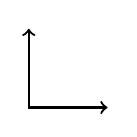
\begin{tikzpicture}[xscale=1, yscale=1]
			\draw [thick, <-> ] (0,1) -- (0,0) -- (1,0);
			\end{tikzpicture}


			\begin{tikzpicture}[xscale=2, yscale=2]
			\draw [thick, <-> ] (0,1) -- (0,0) -- (1,0);
			\end{tikzpicture}
			\end{example}

			\begin{tikzpicture}[xscale=2.5, yscale=2.5]
			\draw [thick, <-> ] (0,1) -- (0,0) -- (1,0);
			\end{tikzpicture}


		\note[item]{}
		\end{frame}















	%	==========================================================
	%		라인 그리기 예제
	%	----------------------------------------------------------
	%		예제
	%	----------------------------------------------------------
		\begin{frame}[t]
		\frametitle{예제 001}



			\begin{example}

				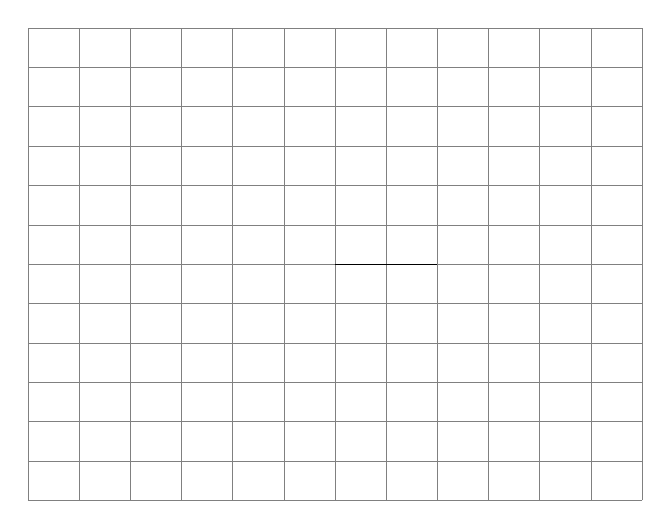
\begin{tikzpicture}[xscale=1.3]
				\draw[help lines, step=.5, color=gray] (-3 , -3) grid ( 3, 3) ;
				\draw (0,0) -- (1,0);
				\end{tikzpicture}

			\end{example}

		\end{frame}


	%	----------------------------------------------------------
	%		예제
	%	----------------------------------------------------------
		\begin{frame}[t]
		\frametitle{예제 001}



			\begin{example}

				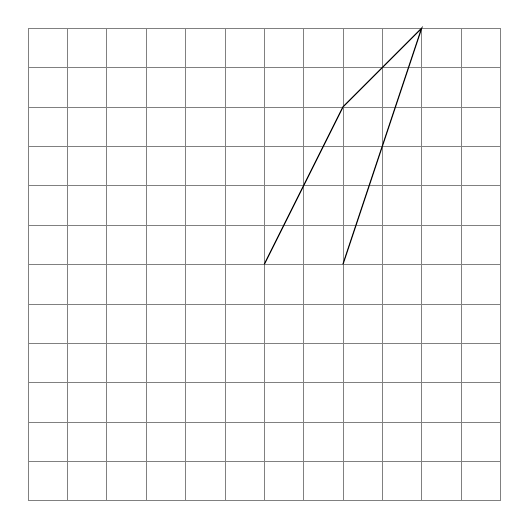
\begin{tikzpicture}[xscale=1.0]
				\draw[help lines, step=.5, color=gray] (-3 , -3) grid ( 3, 3) ;
				\draw (0,0) -- (1,2) -- (2,3) -- (1,0);
				\end{tikzpicture}

			\end{example}

		\end{frame}




	%	----------------------------------------------------------
	%		예제
	%	----------------------------------------------------------
		\begin{frame}[t]
		\frametitle{예제 001}

			\begin{example}

				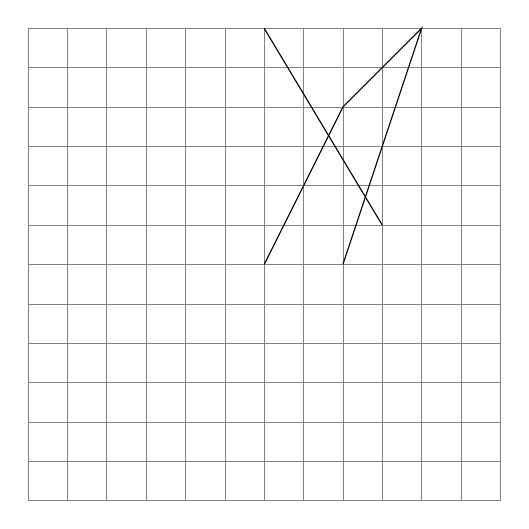
\begin{tikzpicture}[xscale=1.0]
				\draw[help lines, step=.5, color=gray] (-3 , -3) grid ( 3, 3) ;
				\draw (0,0) -- (1,2) -- (2,3) -- (1,0);
				\draw (0,3) -- (1.5,0.5);
				\end{tikzpicture}

			\end{example}

		\end{frame}


	%	==========================================================
	%		예제 : 선의 끝부분 형태
	%	----------------------------------------------------------
		\begin{frame}[t]
		\frametitle{예제 001}

			\begin{example}

				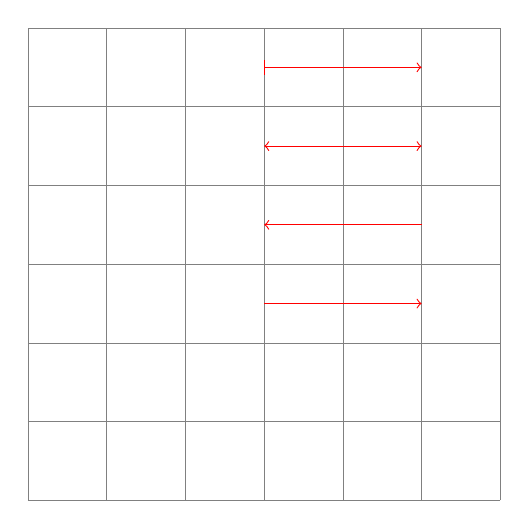
\begin{tikzpicture}[xscale=1.0]
				\draw[help lines, step=1.0, color=gray] (-3 , -3) grid ( 3, 3) ;
				\draw [->] 	[draw=red] (0,-0.5) -- (2,-0.5);
				\draw [<-]	[draw=red] (0,0.5) -- (2,0.5);
				\draw [<->]	[draw=red] (0,1.5) -- (2,1.5);
				\draw [|->]	[draw=red] (0,2.5) -- (2,2.5);
				\end{tikzpicture}

			\end{example}

		\end{frame}



	%	----------------------------------------------------------
	%		예제 : 선의 끝부분 형태지정을 활용한 좌표축 그림
	%	----------------------------------------------------------
		\begin{frame}[t]
		\frametitle{예제 001}

			\begin{example}

				\begin{tikzpicture}[xscale=1.0]
				\draw [<->] 	[draw=red] (0,4) -- (0,0) -- (4,0);
				\end{tikzpicture}

			\end{example}

		\end{frame}


	%	==========================================================
	%		예제 : 선의 두께
	%	----------------------------------------------------------
		\begin{frame}[t]
		\frametitle{예제 : 선의 두께}

			\begin{example}

				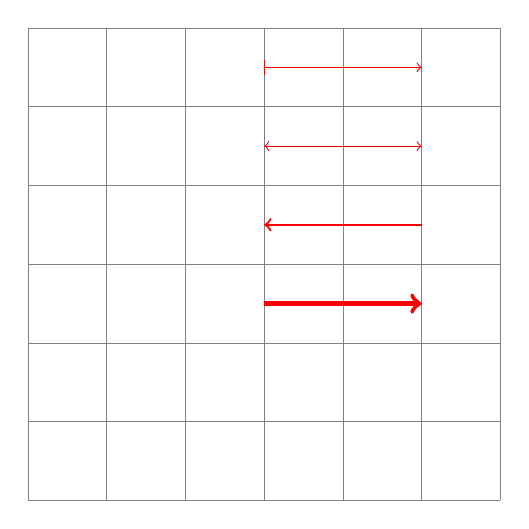
\begin{tikzpicture}[xscale=1.0]
				\draw[help lines, step=1.0, color=gray] (-3 , -3) grid ( 3, 3) ;
				\draw [->] 	[ultra thick	, draw=red] (0,-0.5) -- (2,-0.5);
				\draw [<-]	[thick 		, draw=red] (0,0.5) -- (2,0.5);
				\draw [<->]	[thin		, draw=red] (0,1.5) -- (2,1.5);
				\draw [|->]	[draw=red] (0,2.5) -- (2,2.5);
				\end{tikzpicture}

			\end{example}

		\end{frame}


	%	----------------------------------------------------------
	%		예제 : 선의 두께
	%	----------------------------------------------------------

		\begin{frame}[t]
		\frametitle{예제 : 선의 두께}

			\begin{block}{선의 두께 종류}
			\begin{description}[12345678901234567890]
			\item	[ultra thin]
			\item 	[very thin]
			\item 	[thin]
			\item 	[semithick]
			\item 	[thick]
			\item 	[very thick]
			\item 	[ultra thick]
			\end{description}
			\end{block}

		\end{frame}


	%	----------------------------------------------------------
	%		예제 : 선의 두께 사용자정의
	%	----------------------------------------------------------
		\begin{frame}[t]
		\frametitle{예제 : 선의 두께 : 사용자 정의}

			\begin{example}

				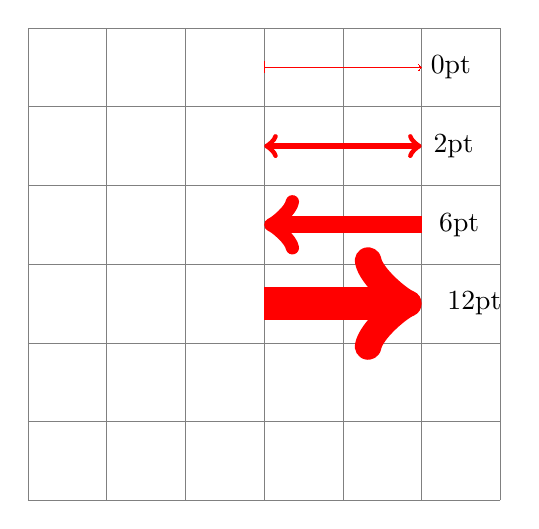
\begin{tikzpicture}[xscale=1.0]
				\draw[help lines, step=1.0, color=gray] (-3 , -3) grid ( 3, 3);
				\draw [->] 	[line width=12pt	, draw=red] (0,-0.5) -- (2,-0.5) 	node [right] {12pt};
				\draw [<-]	[line width=6pt	, draw=red] (0,0.5) -- (2,0.5)		node [right] {6pt};
				\draw [<->]	[line width=2pt	, draw=red] (0,1.5) -- (2,1.5)		node [right] {2pt};
				\draw [|->]	[line width=0pt	, draw=red] (0,2.5) -- (2,2.5)		node [right] {0pt};
				\end{tikzpicture}

			\end{example}

		\end{frame}




	%	==========================================================
	%		예제 : 선의 종류 : 데쉬와 도트
	%	----------------------------------------------------------
		\begin{frame}[t]
		\frametitle{예제 : 선의 종류 : 데쉬와 도트}

			\begin{example}

				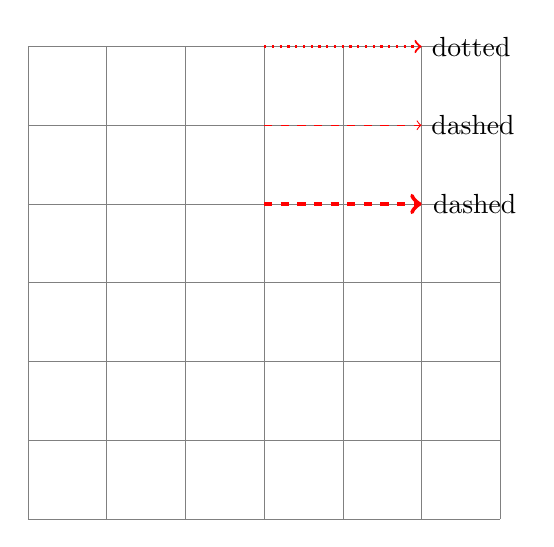
\begin{tikzpicture}[xscale=1.0]
				\draw[help lines, step=1.0, color=gray] (-3 , -3) grid ( 3, 3);
				\draw [->] 	[dashed	,ultra thick	, draw=red] (0,1) -- (2,1) 	node [right] {dashed};
				\draw [->] 	[dashed				, draw=red] (0,2) -- (2,2) 	node [right] {dashed};
				\draw [->] 	[dotted	,thick		, draw=red] (0,3) -- (2,3) 	node [right] {dotted};
				\end{tikzpicture}

			\end{example}

		\end{frame}



	%	----------------------------------------------------------
	%		예제 : 선의 색깔
	%	----------------------------------------------------------
		\begin{frame}[t]
		\frametitle{예제 : 선의 색깔}

			\begin{example}

				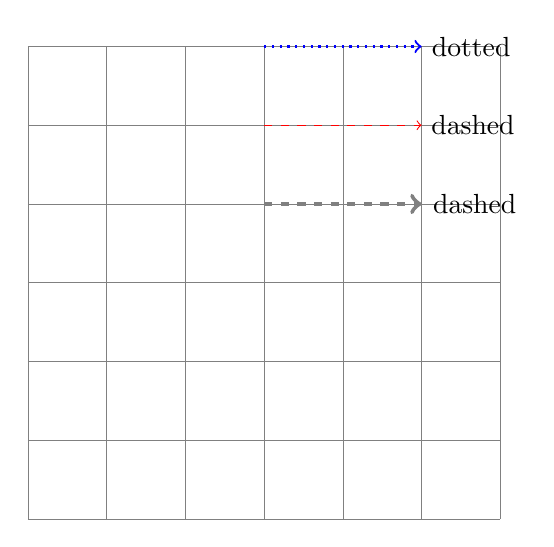
\begin{tikzpicture}[xscale=1.0]
				\draw[help lines, step=1.0, color=gray] (-3 , -3) grid ( 3, 3);
				\draw [->] 	[dashed	,ultra thick	, draw=gray] (0,1) -- (2,1) 	node [right] {dashed};
				\draw [->] 	[dashed				, draw=red] (0,2) -- (2,2) 	node [right] {dashed};
				\draw [->] 	[dotted	,thick		, draw=blue] (0,3) -- (2,3) 	node [right] {dotted};
				\end{tikzpicture}

			\end{example}

		\end{frame}




	%	==========================================================
	%		예제 : 선의 색깔
	%	----------------------------------------------------------

		\begin{frame}[t, shrink=1]
		\frametitle{예제 : 선의 색깔}
				

			\begin{block}{선의 색깔 종류}
			\begin{description}[12345678901234567890]
			\item	[red]		
\begin{tikzpicture}  \draw [->] [ultra thick	, draw=red] (0,1) -- (2,1); \end{tikzpicture}
			\item 	[green]		
\begin{tikzpicture}  \draw [->] [ultra thick	, draw=green] (0,1) -- (2,1); \end{tikzpicture}
			\item 	[blue]		
\begin{tikzpicture}  \draw [->] [ultra thick	, draw=blue] (0,1) -- (2,1); \end{tikzpicture}
			\item 	[cyan]		
\begin{tikzpicture}  \draw [->] [ultra thick	, draw=cyan] (0,1) -- (2,1); \end{tikzpicture}
			\item 	[magenta]		
\begin{tikzpicture}  \draw [->] [ultra thick	, draw=magenta] (0,1) -- (2,1); \end{tikzpicture}
			\item 	[yellow]		
\begin{tikzpicture}  \draw [->] [ultra thick	, draw=yellow] (0,1) -- (2,1); \end{tikzpicture}
			\item 	[black]		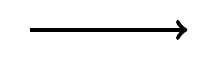
\begin{tikzpicture}  \draw [->] [ultra thick	, draw=black] (0,1) -- (2,1); \end{tikzpicture}
			\item 	[gray]		
\begin{tikzpicture}  \draw [->] [ultra thick	, draw=gray] (0,1) -- (2,1); \end{tikzpicture}
			\item 	[darkgray]	
\begin{tikzpicture}  \draw [->] [ultra thick	, draw=darkgray] (0,1) -- (2,1); \end{tikzpicture}
			\item 	[lightgray]	
\begin{tikzpicture}  \draw [->] [ultra thick	, draw=lightgray] (0,1) -- (2,1); \end{tikzpicture}
			\item 	[brown]		
\begin{tikzpicture}  \draw [->] [ultra thick	, draw=brown] (0,1) -- (2,1); \end{tikzpicture}
			\item 	[lime]		
\begin{tikzpicture}  \draw [->] [ultra thick	, draw=lime] (0,1) -- (2,1); \end{tikzpicture}
			\item 	[olive]		
\begin{tikzpicture}  \draw [->] [ultra thick	, draw=olive] (0,1) -- (2,1); \end{tikzpicture}
			\item 	[orange]		
\begin{tikzpicture}  \draw [->] [ultra thick	, draw=orange] (0,1) -- (2,1); \end{tikzpicture}
			\item 	[pink]		
\begin{tikzpicture}  \draw [->] [ultra thick	, draw=pink] (0,1) -- (2,1); \end{tikzpicture}
			\item 	[purple]		
\begin{tikzpicture}  \draw [->] [ultra thick	, draw=purple] (0,1) -- (2,1); \end{tikzpicture}
			\item 	[teal]		
\begin{tikzpicture}  \draw [->] [ultra thick	, draw=teal] (0,1) -- (2,1); \end{tikzpicture}
			\item 	[violet]		
\begin{tikzpicture}  \draw [->] [ultra thick	, draw=violet] (0,1) -- (2,1); \end{tikzpicture}
			\item 	[white]		\begin{tikzpicture}  \draw [->] [ultra thick	, draw=white] (0,1) -- (2,1); \end{tikzpicture}
			\end{description}
			\end{block}

		\end{frame}





	%	==========================================================
	%		커브 그리기 예제
	%	----------------------------------------------------------
	%		예제
	%	----------------------------------------------------------

		\begin{frame}[t]
		\frametitle{예제 : 사각형 그리기 예제}

			\begin{example}

				\begin{tikzpicture}[xscale=1.0]
				\draw [blue] (0,0) rectangle (2,4);
				\end{tikzpicture}

			\end{example}

		\end{frame}


	%	----------------------------------------------------------
	%		예제
	%	----------------------------------------------------------

		\begin{frame}[t]
		\frametitle{예제 : 원 그리기 예제}

			\begin{example}

				\begin{tikzpicture}[xscale=1.0]
				\draw [blue] (0,0) circle [radius=3];
				\end{tikzpicture}

			\end{example}

		\end{frame}


	%	----------------------------------------------------------
	%		예제
	%	----------------------------------------------------------

		\begin{frame}[t]
		\frametitle{예제 : 호 그리기 예제}

			\begin{example}

				\begin{tikzpicture}[xscale=1.0]
				\draw [blue] (0,0) arc [radius=3, start angle=45, end angle=120 ];
				\end{tikzpicture}

			\end{example}

		\end{frame}



	%	----------------------------------------------------------
	%		예제 : rounded corners
	%	----------------------------------------------------------

		\begin{frame}[t]
		\frametitle{예제 : rounded corners}

			\begin{example}

				\begin{tikzpicture}[xscale=1.0]
				\draw [<->, rounded corners, thick, purple] (0,4) -- (0,0) -- (6,0);
				\end{tikzpicture}

			\end{example}

		\end{frame}



	%	==========================================================
	%		예제
	%	----------------------------------------------------------
		\begin{frame}[t]
		\frametitle{예제 001}



			\begin{example}

				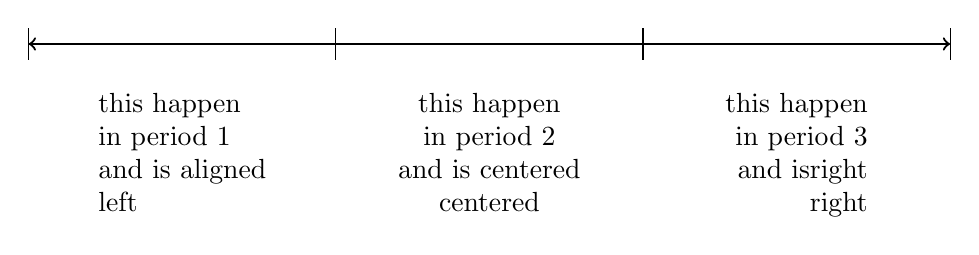
\begin{tikzpicture}[xscale=1.3]
				\draw [thick, <-> ] (0,0) -- (9,0);
				\draw (0,-0.2) -- (0,0.2);
				\draw (3,-0.2) -- (3,0.2);
				\draw (6,-0.2) -- (6,0.2);
				\draw (9,-0.2) -- (9,0.2);
				\node[align=left, below] 	at (1.5,-0.5) {this happen \\in period 1 \\and is aligned \\left};
				\node[align=center, below] 	at (4.5,-0.5) {this happen \\in period 2 \\and is centered \\centered};
				\node[align=right, below] 	at (7.5,-0.5) {this happen \\in period 3 \\and isright \\right};

				\end{tikzpicture}

			\end{example}

		\end{frame}


	%	==========================================================
	%		예제
	%	----------------------------------------------------------
		\begin{frame}[t]
		\frametitle{예제 002}



			\begin{example}

				
\begin{tikzpicture}
				\draw [-> ] (0,0) -- (2,0);
				\node [right] 	at (2.0,0.0) {above below};
				\end{tikzpicture}

			\end{example}

		\end{frame}



	%	==========================================================
	%		예제
	%	----------------------------------------------------------
		\begin{frame}[t]
		\frametitle{예제 003}



			\begin{example}

				\begin{center}
				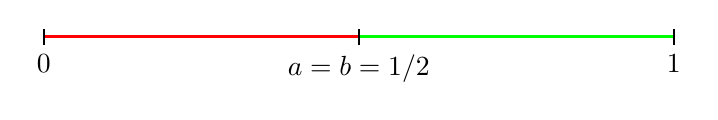
\begin{tikzpicture}[xscale=8]
				\draw [-] [draw=red, very thick] 		(0,0) -- (0.5,0);
				\draw [-] [draw=green, very thick] 	(0.5,0) -- (1,0);

				\draw [thick]	(0,-0.1)   node [below]{0}         -- (0,0.1);
				\draw [thick]	(0.5,-0.1) node [below]{$a=b=1/2$} -- (0.5,0.1);
				\draw [thick]	(1,-0.1)   node [below]{1}         -- (1,0.1);

				\end{tikzpicture}
				\end{center}

			\end{example}

		\end{frame}



		% 스케일 명령이 주어도 문자는 스케일 되지 않음


	%	==========================================================
	%		예제
	%	----------------------------------------------------------
		\begin{frame}[t]
		\frametitle{예제 004}



			\begin{example}

				\begin{center}
				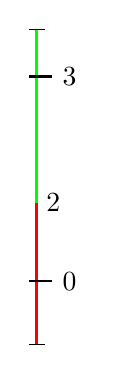
\begin{tikzpicture}[yscale=4]
				\draw [-] [draw=red, very thick] 	    (0.0,0.00) -- (0,0.45);
				\draw [-] [draw=green, very thick] 	    (0.0,0.45) -- (0,1.00);

				\draw [thick]	(-0.1,0.2) -- (0.2,0.2) node [align=left, right]{0};
				\node [right]	at (0.0,0.45){2};
				\draw [thick]	(-0.1,0.85) -- (0.2,0.85) node [align=left, right]{3};


				\draw (-0.1,0.00) -- (0.1,0.00);
				\draw (-0.1,1.00) -- (0.1,1.00);

				\end{tikzpicture}
				\end{center}

			\end{example}

		\end{frame}



















% ------------------------------------------------------------------------------
% End document
% ------------------------------------------------------------------------------
\end{document}


